\chapter{General discussion and synthesis}
%\addcontentsline{toc}{chapter}{Chapter 6}
%\markboth{}{Thesis Synthesis}
\label{C06}

\section{Summary of main findings}
\label{C06_01}

The overarching goal of this thesis was to investigate how local biodiversity is impacted by land changes in the past and whether those impacts vary with key attributes of land change (\eg magnitude, frequency, time passed or sequence), across taxonomic groups, and geographic regions. I found past differences in land-surface conditions to be more important in explaining local species assemblage composition than current differences (Chapter \ref{C02}). After an abrupt land change and depending on attributes of land change, local species richness and total abundance were reduced, and assemblage composition altered (Chapter \ref{C03}) but were often able to recover to levels comparable to unchanged sites. Using the same biodiversity data, I found local biodiversity measures to decrease following past land-cover change and that attributes of land-cover change influence local, national and global biodiversity estimates differently (Chapter \ref{C04}). Chapters \ref{C02}-\ref{C04} assessed whether past land changes are correlated with spatial differences in local biodiversity at one point in time, however the impacts on biodiversity change \textit{per se} were not assessed. The results in chapter \ref{C05} indicated that past and concurrent landscape-wide land changes are correlated with but explain on average little variation in local bird diversity change. Overall these results demonstrate the pervasive impacts land changes can have on local biodiversity globally. In the following I discuss the implications of these results and directions for future research.

\section{Applications and limitations of findings}
\label{C06_02}

In this thesis, I attempted to establish links between local biodiversity data (Projecting Responses of Ecological Diversity In Changing Terrestrial Systems [\textbf{PREDICTS}] \textendash\ \cite{Hudson2016}; United States Breeding Bird Survey [\textbf{BBS}] \textendash\ \cite{Pardieck2018}) and estimates of land change quantified from remotely-sensed satellite data globally (Figure \ref{F01_01}). This allowed me to address three important knowledge gaps.

First, most previous broad-scale studies only considered superficially \textendash\ if at all \textendash\ land changes in the past \citep{Alkemade2009,Murphy2014,Newbold2015} and corresponding biotic lag effects on local biodiversity \citep{Dullinger2013,Hylander2013}. Throughout the thesis and regardless of how past land changes were quantified (Chapter \ref{C02}-\ref{C05}), I discovered a consistent pattern that land changes in the past on average influenced local biodiversity measures and altered species assemblage composition, often more so than concurrent differences of land-surface conditions (Chapter \ref{C02} \& \ref{C05}). This implies \textendash\ not surprisingly given existing evidence of lasting influences of past land change on biodiversity \citep{Foster2003,Ewers2013,Perring2015} \textendash\ that previous broad-scales syntheses \citep{Murphy2014,Newbold2015,Alroy2017} likely underestimated the impacts of land change on local biodiversity. 

The second main gap this thesis addressed is the explicit consideration of attributes of land change. Land changes can be diverse and difficult to quantify and compare \citep{Kleyer2007}. Theoretical frameworks, such as the one developed by \cite{Watson2014}, distinguish land changes by a set of key attributes (\eg magnitude, frequency, time passed or sequence) with clear ecological relevance. Local biodiversity measures were considerably reduced following land changes with large magnitude (Chapter \ref{C03} \& \ref{C05}), \eg clear cutting of forested land or urbanization, which can act as disturbance \citep{Scheffer2001,Scheffer2003} reducing ecosystem stability \citep{Pimm1984,Hautier2015} and local biodiversity in concurrent and future years. In addition, the cumulative frequency of land changes (Chapter \ref{C02} \& \ref{C05}) can also influence biodiversity change, which \textendash\ together with magnitude impacts \textendash\ can be applied to improve predictions of biodiversity change \citep{Ewers2009,Ewers2013} and to establish linear and non-linear thresholds after which biodiversity change tends to accelerate \citep{VanderHoek2013,Gutzwiller2015}. Moreover, the results indicate that local biodiversity measures can \textendash\ on average \textendash\ recover to levels comparable of unchanged sites (Chapter \ref{C03} \& \ref{C04}), which is an important finding given that biodiversity recovery from past land changes is of major biodiversity conservation concern globally, especially as more and more land is secondary vegetation \citep{Chazdon2003,Jones2018}. Lastly, this thesis found that impacts of past land-cover change differed depending on the sequence of land cover (Chapter \ref{C04}), extending our knowledge on these impacts relative to previous studies that investigated only specific land-cover sequences or were based on very few estimates \citep{Foster2003,Bremer2010,Watson2014}.

Third, the influence of past land change on local biodiversity was previously unknown across geographic regions, taxonomic groups and biodiversity measures. I demonstrate how remotely-sensed estimates of land change can be robustly linked to local biodiversity data. Some attributes of land change, \eg time passed \citep{Martin2013,Fu2017} and magnitude \citep{Shackelford2017}, have been investigated previously in broad-scale syntheses. However, those studies lacked the taxonomic and geographic breadth, had small sample sizes \textendash\ 14 studies in the case of \cite{Shackelford2017} \textendash\ and were predominantly based on species richness only, which can be a misleading measure of biodiversity \citep{Su2004,Hillebrand2017}. The results in this thesis demonstrate that past land changes continue to influence local biodiversity globally and across multiple taxonomic groups and measures of local biodiversity (Chapter \ref{C02}-\ref{C05}). Furthermore, by using satellite-based instead of study-derived estimates of land change, the results presented in this thesis can easily be verified, repeated or build on by future studies. 

\subsection{Limitations of the presented results}
\label{C06_0102}

This thesis relies exclusively on a remote-sensing based characterization of land change. The definition of land change recognizes that land-use and/or land-cover cannot easily be separated \citep{Turner2007}. For instance, the observed differences in land-surface conditions in chapter \ref{C02} could be caused by changes in land use and/or land cover, with the exact driver being unknown. Land change can be driven by natural \textendash\ rather than anthropogenic \textendash\ factors and I did not attempt to identify the drivers of land change \citep{Curtis2018}. However, it could be that land changes caused by natural factors \textendash\ \eg precipitation anomalies, flooding, etc. \textendash\ compared to anthropogenically caused land changes \textendash\ \eg agricultural intensification or urbanisation \textendash\ have differing impacts on local biodiversity.

Although remote sensing data has great potential as a predictor in biodiversity models \citep{Petrou2015,Lausch2016}, there are temporal limits in data availability, particularly before the 1970s for satellite data and the 1910s for regional aerial photographs. Since the temporal availability of satellite-based remote-sensing data limits the reference baseline of this thesis, it is likely that some of the largest impacts on local biodiversity globally, \eg those anthropogenically-driven pressures responsible for reducing biodiversity intactness globally \citep{Newbold2016a}, are likely being missed \citep{Mihoub2017}, making our estimates conservative.

A lack of explanatory power \textendash\ both exploratory and for prediction \textendash\ increases uncertainty. The results presented here consistently indicate that attributes of past land change are correlated with spatial and temporal differences in local biodiversity (Chapter \ref{C02}-\ref{C05}), however the amount of explained variance (R\textsuperscript{2}) of past land changes is relatively low (\textasciitilde 1.4\% in Chapter \ref{C02} or 5\% to 12\% in Chapter \ref{C05}). This can be a limitation of the models constructed particularly if they are used to predict local biodiversity responses in novel, \eg unsampled, geographic regions \citep{Jung2016}, where prediction uncertainty can be quite large (Figure \ref{F04_04} in Chapter \ref{C04}). However, the explained variance is similar to that of other studies on the same dataset, typically lying between 2\% and 11\% for PREDICTS data \citep{Newbold2014b,DePalma2015,Jung2016} or 2.5\% to 5.4\% (the average R\textsuperscript{2}) in ecological meta-analyses \citep{Moller2002}. It is likely that this is a general issue of broad-scale syntheses and future studies should consider investigating this further, for instance through independent validations and the development of methodological improvements (see \ref{C06_0401}).

\section{Broader implications}
\label{C06_03}
\subsection{Impacts on ecosystem functioning}
\label{C06_0301}

Why are impacts of past land change important to consider? A loss of local biodiversity can lead to reduced ecosystem functions and services \citep{Cardinale2012,Albrecht2014,Oliver2015b}, especially if functionally non-redundant species or large proportions of the original species assemblage are lost \citep{Oliver2015}. The results presented in this thesis indicate that local biodiversity measures were predominantly reduced and/or altered after a past land change (Chapter \ref{C02}-\ref{C05}) and it is likely that these impacts affect ecosystem functioning and ultimately human wellbeing \citep{Cardinale2012}. A previous study demonstrated that the biodiversity intactness index (BII) \textendash\ an index with direct links to ecosystem functioning \textendash\ has been reduced across terrestrial biomes because of differences in land use and/or land cover \citep{Newbold2016a}. However, these global BII estimates do not incorporate lasting impacts of past land changes and subsequent reductions in the BII may cause a “ecosystem service debt” \citep{Isbell2015}. I found local biodiversity to be able to recover to levels comparable to unchanged sites within a few years (Chapter \ref{C03}-\ref{C04}), which implies that ecosystem functions affected by land change might be able to recover relatively quickly. 

\subsection{Implications for conservation policy}
\label{C06_0302}

Global biodiversity models are a useful tool for creating spatial and temporal projections of biodiversity change \citep{Pereira2010,Harfoot2014,Purvis2018}. Biodiversity projections can be used to predict plausible outcomes of policy interventions and make recommendations how to mitigate the ongoing global biodiversity loss \citep{Mace2018}. It has been argued that global projections of biodiversity change neglect future land changes \citep{Titeux2016}, and in addition they also ignore lasting impacts of past land changes. No regional or global assessment for the Intergovernmental Science-Policy Platform on Biodiversity and Ecosystem Services (IPBES) currently considers lasting influences of past land change on biodiversity. This thesis demonstrates that local biodiversity is consistently influenced by past land change (Chapter \ref{C02}-\ref{C05}) through biotic lag effects and suggests that future, more accurate projections of biodiversity change should incorporate lasting impacts of past land changes. 

There are several key points that can serve as recommendations for future biodiversity projections and policy outputs: The results presented show (\textit{i}) how temporally explicit land change estimates from remote sensing data can be robustly linked to local biodiversity data on a global scale, thus providing an opportunity to incorporate these estimates into existing modelling frameworks such as PREDICTS \citep{Newbold2015,Newbold2016a,Purvis2018} or GLOBIO \citep{Alkemade2009}; (\textit{ii}) that land changes in the past have lasting impacts on biodiversity globally and thus should be considered in biodiversity projections. Policy-relevant indices \textendash\ such as the biodiversity intactness index \citep{Newbold2016a,Purvis2018} \textendash\ could be adapted so that lasting impacts of past land changes are incorporated; (\textit{iii}) The results presented show a number of approaches for assessing land change that could be quantified as spatial-temporal maps \textendash\ \ie the dissimilarity in annual vegetation dynamics (Chapter \ref{C02}) or the magnitude of abrupt land changes (Chapter \ref{C03} \& \ref{C05}) \textendash\ and potentially serve as remotely-sensed essential biodiversity variables (RS-EBV), a group of biodiversity and policy relevant variables purely defined from remote sensing \citep{Skidmore2015,Lausch2016}.

\section{Recommendations for future research}
\label{C06_04}
\subsection{Improving predictability of impacts of land change}
\label{C06_0401}

Biodiversity models can be useful to quantify the global impacts of land change and create predictive projections of future expected impacts \citep{Purvis2018}. The explained variance of these models is not only an indicator for the strength of research findings, but also important to consider for predictions, particularly so in novel environments \citep{Yates2018}. Transferability is defined as the “capacity of a model to produce accurate and precise predictions for a new set of predictors that differ from those on which the model was trained” \citep{Yates2018}. This is especially relevant if impacts of land change on local biodiversity are projected globally across unsampled regions \citep{Newbold2015,Purvis2018}, ignoring spatial and temporal biases in local biodiversity databases \citep{Martin2012,Hudson2014,Gonzalez2016}. Future studies should (\textit{i}) investigate whether predicted impacts of land change are consistent in novel environments \citep{Yates2018}. This can be achieved for instance by using independently collected biodiversity data for comparison and validation \citep{Jung2016}, (\textit{ii}) by seeking ways to incorporate prediction uncertainty into biodiversity projections, similar to what was done visually in chapter \ref{C04} of this thesis and (\textit{iii}) investigate ways how hierarchical models \textendash\ particularly those used by PREDICTS \citep{Purvis2018} \textendash\ can be improved, for instance by better accounting for differences in sampling methodology, effort and spatial extent.  

\subsection{Interactions between attributes of land change}
\label{C06_0402}

The theoretical framework by \cite{Watson2014} distinguishes four attributes of land change, however it does not consider interactions between those attributes. Given that shifts in magnitude are common and vary in frequency for many agricultural landscapes \citep{Kleyer2007}, it is likely that interacting attributes of land change impact local biodiversity differently. Previous studies have hypothesized that impacts of land change of large magnitude likely vary with time passed and affect biodiversity recovery \citep{Shackelford2017}. Similarly, local biodiversity recovery with time passed might differ depending on the sequence in land-cover \citep{Chazdon2003,Martin2013}. The work presented in this thesis used some of the most extensive, currently available local biodiversity datasets, representing \textasciitilde 1\% of all formally described species in the case of PREDICTS \citep{Hudson2016}, and the longest timeseries, with over 34 years of continuous sampling, in the case of the BBS \citep[, Figure \ref{F01_01}]{Pardieck2018}. Despite these taxonomically broad and temporally long databases, data limitations made testing for interactive effects between attributes of land change not feasible in the analyses. Future studies could (\textit{i}) utilize modelling approaches less dependent on minimal sample size, \eg Bayesian hierarchical models with informative priors \citep{Iknayan2014} or (\textit{ii}) collect additional biodiversity (see \ref{C06_0403}) and remote sensing data (\ref{C06_0404}). Depending on data availability, future studies could attempt to combine the approaches presented in this thesis, \ie to test for the influence of shifts in magnitude across varying land-cover sequences and/or time passed, which would further improve our understanding of the lasting impacts of land change.

\subsection{Improving availability of biodiversity data}
\label{C06_0403}

Quantifying the impacts of land change on local biodiversity remains a challenge. Most of the work presented in this thesis (Chapter \ref{C02}-\ref{C04}) inferred the impacts of past land change on local biodiversity using matched spatial pairs of sites. While this approach is robust and well established \citep{Purvis2018}, it misses biodiversity dynamics and can be misleading if reference sites are not appropriate or affected by other unmeasured variables \citep{Franca2016,Jung2016,DePalma2018}. Biodiversity time series, such as those from long-term monitoring schemes such as the BBS \citep{Pardieck2018} or global databases \citep[\eg BioTime, ][]{Dornelas2018}, can provide valuable alternatives to study the impacts of land change on local biodiversity. Observed impacts of land change on local biodiversity over recent years might be conservative as the regional species pool in many areas of the world was likely already depleted decades or centuries before local biodiversity sampling and before satellite-based remote sensing data became available \citep{Newbold2016a,Mihoub2017}. In addition, existing biodiversity time series often underrepresent regions where contemporary drivers of biodiversity change are most intense \citep{Gonzalez2016,Cardinale2018}. Overall there is a need to improve both quality and quantity of biodiversity data suitable to test for the impacts of land change.

% ---------------- Figure 1 --------------------- %
\begin{figure}[ht]
\centering
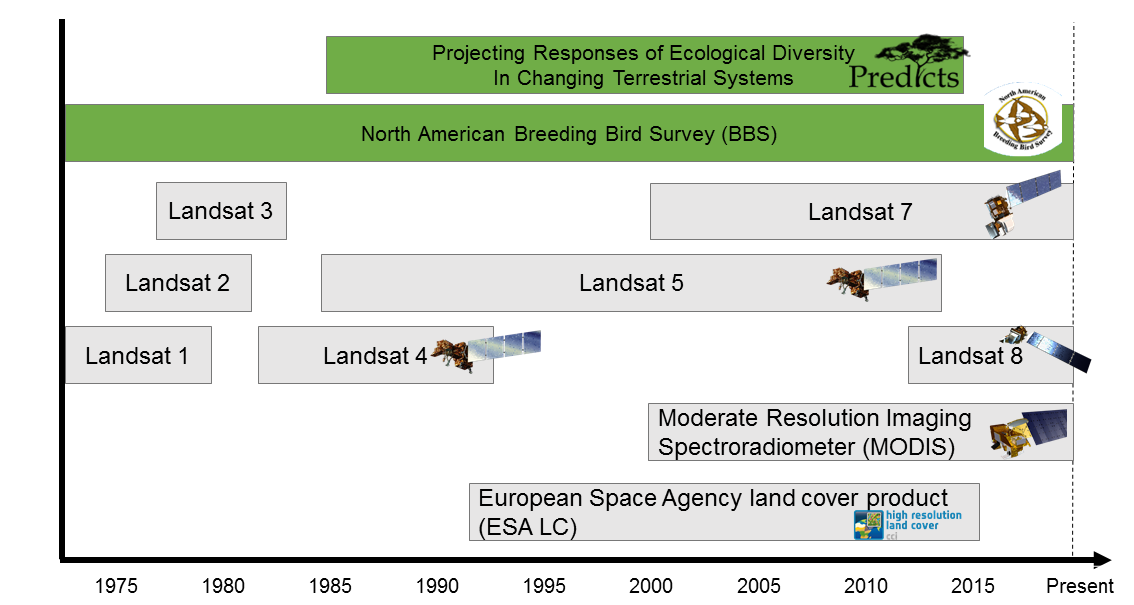
\includegraphics[width=.8\textwidth]{chapter6/F01}
\caption{ Remote sensing data can help identify areas suitable for resampling of local biodiversity. Combining sites from the PREDICTS project (Chapter \ref{C02}-\ref{C04}) and time series of land cover \citep{ESA2017}, I assessed whether land cover has changed after biodiversity sampling (\textbf{a}) PREDICTS sites (394 sites, 115 studies) with a land-cover change after biodiversity had been sampled (average 5.57 $\pm$ 3.3 SD years) according to the ESA LC product \citep{ESA2017}. Colours and y-axis indicate the land cover at the time of biodiversity sampling. The x-axis shows the years the site remained in a given land cover (mean estimate and standard deviation shown as dots and error bars) before a land-cover change occurred. Numbers show the total number of sites. (\textbf{b}) Example of a PREDICTS site which was forest-covered at the time of biodiversity sampling in 2003 but was converted to agriculture seven years later. (\textbf{c}) Flow diagram showing the land-cover sequences observed for sites with a post-sampling land-cover change.}
\label{F06_01}
\end{figure}
% -------------------------------------------- %

To infer how land change impacts local biodiversity, specific sampling designs are necessary \citep{DePalma2018}. The best way of assessing the impacts of land change on biodiversity is a before-after-control-impact (BACI) study design \citep{Cardinale2018,DePalma2018}. Data from multiple BACI studies could be used to quantify the immediate difference in local biodiversity after land change \citep{Ratajczak2018}, taking attributes of land change \citep{Watson2014}, site-specific local factors \citep{Jung2016} and variability among species assemblages \citep{Dornelas2013,Franca2016} into account. However, such BACI data are currently not readily available. A new phase of the PREDICTS project (labelled PREDICTS-2) aims to systematically collect estimates of local biodiversity before and after land change. Remote sensing data \textendash\ either using a land change detection algorithm (Chapter \ref{C03}) or readily available land cover products (Chapter \ref{C04}) \textendash\ can help to identify sites where land cover has or has not changed after local biodiversity sampling (Figure \ref{F06_01}). There is an opportunity to sample those sites again \textendash\ preferably using identical methods and observers \textendash\ to obtain BACI estimates of local biodiversity in response to land change \citep{DePalma2018}. Such data would further improve our understanding of the impacts of land change on local biodiversity.

\subsection{Improving availability of remotely-sensed estimates of land change}
\label{C06_0404}

The availability and accessibility of remote sensing data continues to improve. The move of the global Landsat archive into the public domain in 2008 enabled unprecedented and free access to satellite imagery \citep{Wulder2015}. Opposed to the early 1990s and 2000s, when mostly single satellite images were analysed in a time-consuming process, modern satellite-based remote sensing analyses increasingly utilize entire time series of satellite imagery \citep{Kennedy2014,Hermosilla2015a}. The development of new land change detection \citep{Coppin2004,Abercrombie2016,Zhu2017} and machine learning algorithms \citep{Maxwell2018}, and the rise of cloud processing environments \citep{Gorelick2017} have further supported the creation of temporally consistent remotely-sensed land cover products globally \citep{ESA2017,Hermosilla2018,Sulla-Menashe2019}. These developments have led some to declare that a new area of land cover analysis has emerged, fittingly called “Land cover 2.0” \citep{Wulder2018}. It is highly likely that future investigations into the impacts of land change on local biodiversity can rely on improved data and algorithm availability.

There are a number of promising avenues for future research linking biodiversity and remotely-sensed land change data: More efforts are needed to (\textit{i}) create and utilize remotely-sensed proxies of land-use change globally, piloted for instance for cropland size \citep{Fritz2015} and yield \citep{Lobell2015}, pasture grazing intensity \citep{Rufin2015,Aguiar2017} or forest plantation rotations \citep{LeMaire2014}; (\textit{ii}) clearly determine natural and anthropogenic drivers of land change, as has recently been done for forests globally \citep{Curtis2018}, (\textit{iii}) consider additional data to extend the available time period \textendash\ such as air borne historical photographs \citep{SZABO2011,Cousins2015} or “legacy” satellite imagery predating the 1980s (\eg Landsat 1-3, Figure \ref{F01_01}), which were not readily available at the time this thesis was conducted.

\section{Concluding remarks}
\label{C06_05}

The impacts of land change on local biodiversity are complex and require looking beyond current differences in land use and/or land cover. Frameworks such as the one developed by \cite{Watson2014} are useful to incorporate attributes of land change into global biodiversity models. The results presented here demonstrate that attributes of past land change impact local biodiversity differently on a global scale and show how remote sensing can be used to quantify spatio-temporal land change. Overall these results show how new insights into local biodiversity patterns can be gained by combining existing data sources.

We live in an age of unprecedented availability of data. This situation provides new opportunities to detect and quantify links between remotely sensed land change and biodiversity data. These opportunities could lead to improved and ultimately near real-time predictions of biodiversity change following land change. However, while technology and data-driven research may assist in providing further evidence and understanding of environmental issues, the preservation of biodiversity is ultimately up to government interventions and societal actions. I hope that quantitative evidence \textendash\ based on data syntheses such as those presented in this thesis \textendash\ will support decision making and that the results of this thesis contribute towards biodiversity conservation.    


\clearpage
%\bibliography{content/04Chapter}

%\appendix
%\begingroup
%  % SI - Figure 1 Missing data
\begin{figure}[h]
\centering
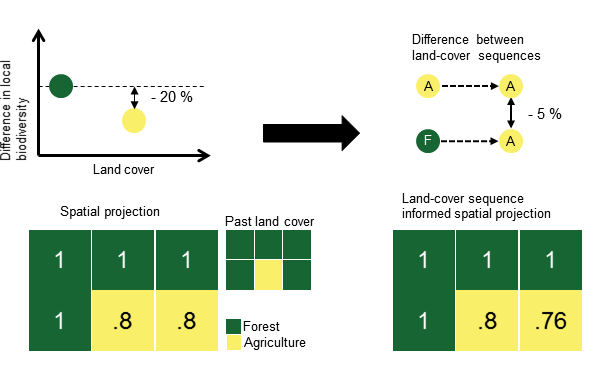
\includegraphics[width=1\textwidth]{chapter3/SI01}
\caption{ Average temporal distribution of Landsat data and an example times series of Landsat data. (\textbf{a}) Distribution of available Enhanced Vegetation Index (EVI) data in years covered by the Landsat missions. Points show the average monthly EVI data availability per year (0 to 12 months of data) across time series and PREDICTS sites grouped by 15\textdegree latitude bins. The size of points indicates the mean data availability (0 to 100\% with 100\% having 12 months of available data in a given year), while the colour shows the number of PREDICTS sites contributing to the mean (as PREDICTS sites were sampled in varying years). (\textbf{b}) Example time series for one PREDICTS site with a high proportion of missing data before 1999. In all analyses such time series were truncated to the period from 1999 onwards (indicated by the dashed line).}
\label{SI03_01}
\end{figure}

% SI - Figure 2 Binning
\begin{figure}[h]
\centering
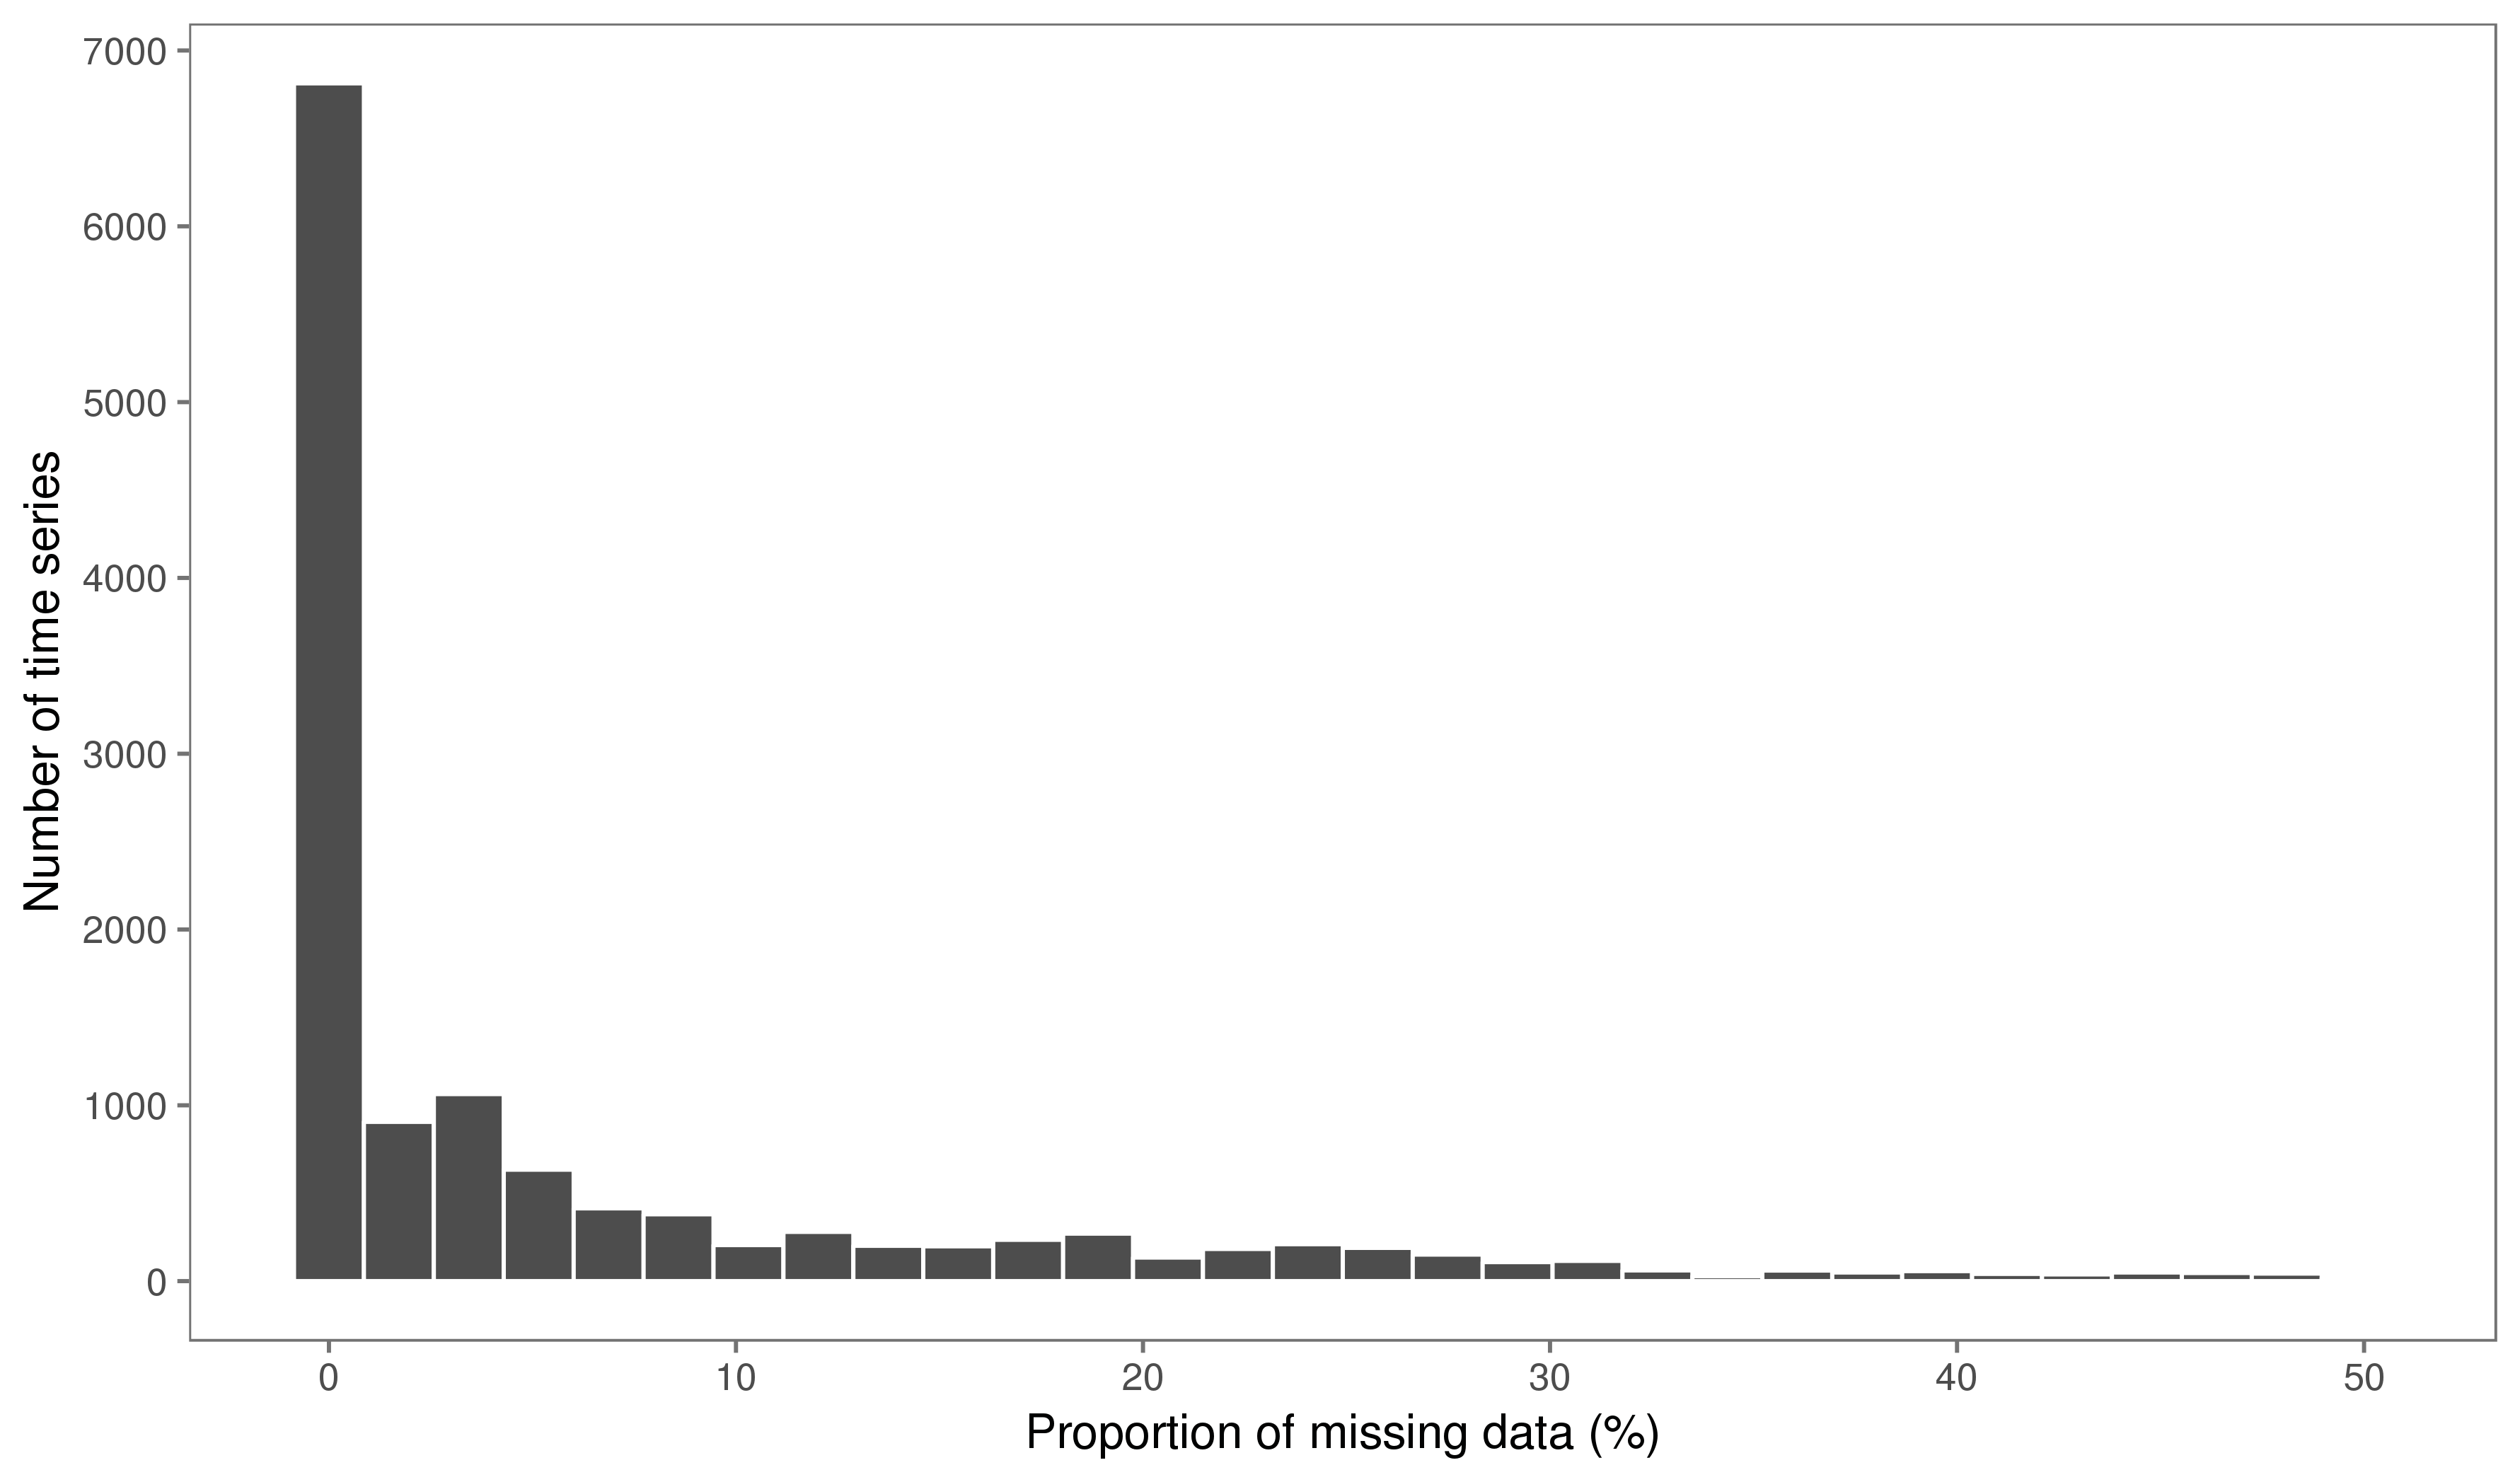
\includegraphics[width=1\textwidth]{chapter3/SI02}
\caption{ Number of sites with abrupt land change per attribute. Number of sites (black line) per attribute of abrupt land change with (\textbf{a}) the relative shift in magnitude, (\textbf{b}) the shift in trend as difference in annual EVI trend, and (\textbf{c}) the time passed between abrupt land change and biodiversity sampling. Background colours in (\textbf{a}) and (\textbf{b}) indicate the binning into six groups for shifts in magnitude (> 50\%, > 25\% to $\leq$ 50\%, and $\leq$ 25\% EVI loss [$---$ to $-$] or gain [$+++$ to $+$]), and in trend (0.01, 0.05, and > 0.05 annual negative [$---$ to $-$] to positive [$+++$ to $+$] EVI trend differences). Gray lines in (\textbf{c}) delineate bins of time passed ($\leq$ 5 years, > 5 and $\leq$ 10 years, and >10 years). Colours as in Figure \ref{F03_02}.}
\label{SI03_02}
\end{figure}

% SI Table 1------ %
% From here https://www.tablesgenerator.com/
\begin{table}[]
\centering
\caption{Number of PREDICTS sites and studies with an abrupt land change. Shown as either a change in magnitude (columns) and/or change in trend (trend). Symbols as in Figure \ref{F03_02}. }
\label{SIT03_01}
\begin{tabular}{@{}lllllllllll@{}}
                                          &                                           & \multicolumn{7}{c}{\textbf{Shift in magnitude}}                                                                                                                                                                    &                               &                             \\
                                          &                                           & \textbf{- - -}             & \textbf{- -}                & \textbf{-}                   & \textbf{0}                    & \textbf{+}                   & \textbf{+ +}                & \textbf{+ + +}              & \textbf{Total sites}          & \textbf{Studies}            \\ \cmidrule(l){3-11} 
                                          & \multicolumn{1}{l|}{- - -}                & 2                          & 8                           & 192                          & NA                            & 73                           & 26                          & 22                          & \cellcolor[HTML]{EFEFEF}323   & \cellcolor[HTML]{C0C0C0}57  \\
                                          & \multicolumn{1}{l|}{- -}                  & 7                          & 281                         & 642                          & NA                            & 497                          & 158                         & 53                          & \cellcolor[HTML]{EFEFEF}1638  & \cellcolor[HTML]{C0C0C0}175 \\
                                          & \multicolumn{1}{l|}{-}                    & 7                          & 88                          & 256                          & NA                            & 231                          & 154                         & 53                          & \cellcolor[HTML]{EFEFEF}789   & \cellcolor[HTML]{C0C0C0}184 \\
                                          & \multicolumn{1}{l|}{0}                    & NA                         & NA                          & NA                           & 10102                         & NA                           & NA                          & NA                          & \cellcolor[HTML]{EFEFEF}10102 & \cellcolor[HTML]{C0C0C0}358 \\
                                          & \multicolumn{1}{l|}{+}                    & 9                          & 102                         & 399                          & NA                            & 410                          & 205                         & 49                          & \cellcolor[HTML]{EFEFEF}1174  & \cellcolor[HTML]{C0C0C0}237 \\
                                          & \multicolumn{1}{l|}{\textbf{+ +}}         & 47                         & 172                         & 342                          & NA                            & 465                          & 254                         & 86                          & \cellcolor[HTML]{EFEFEF}1366  & \cellcolor[HTML]{C0C0C0}224 \\
\multirow{-7}{*}{\textbf{\rotatebox{90}{Shift in trend}}} & \multicolumn{1}{l|}{\textbf{+ + +}}       & 12                         & 137                         & 47                           & NA                            & 34                           & 12                          & 31                          & \cellcolor[HTML]{EFEFEF}273   & \cellcolor[HTML]{C0C0C0}56  \\
                                          & \multicolumn{1}{l|}{\textbf{Total sites}} & \cellcolor[HTML]{EFEFEF}84 & \cellcolor[HTML]{EFEFEF}788 & \cellcolor[HTML]{EFEFEF}1878 & \cellcolor[HTML]{EFEFEF}10102 & \cellcolor[HTML]{EFEFEF}1710 & \cellcolor[HTML]{EFEFEF}809 & \cellcolor[HTML]{EFEFEF}294 &                               &                             \\
                                          & \multicolumn{1}{c|}{\textbf{Studies}}     & \cellcolor[HTML]{C0C0C0}34 & \cellcolor[HTML]{C0C0C0}135 & \cellcolor[HTML]{C0C0C0}246  & \cellcolor[HTML]{C0C0C0}358   & \cellcolor[HTML]{C0C0C0}263  & \cellcolor[HTML]{C0C0C0}171 & \cellcolor[HTML]{C0C0C0}83  &                               &                            
\end{tabular}
\end{table}
% ------ %

% SI - Figure 3 Cross-correlations
\begin{figure}[h]
\centering
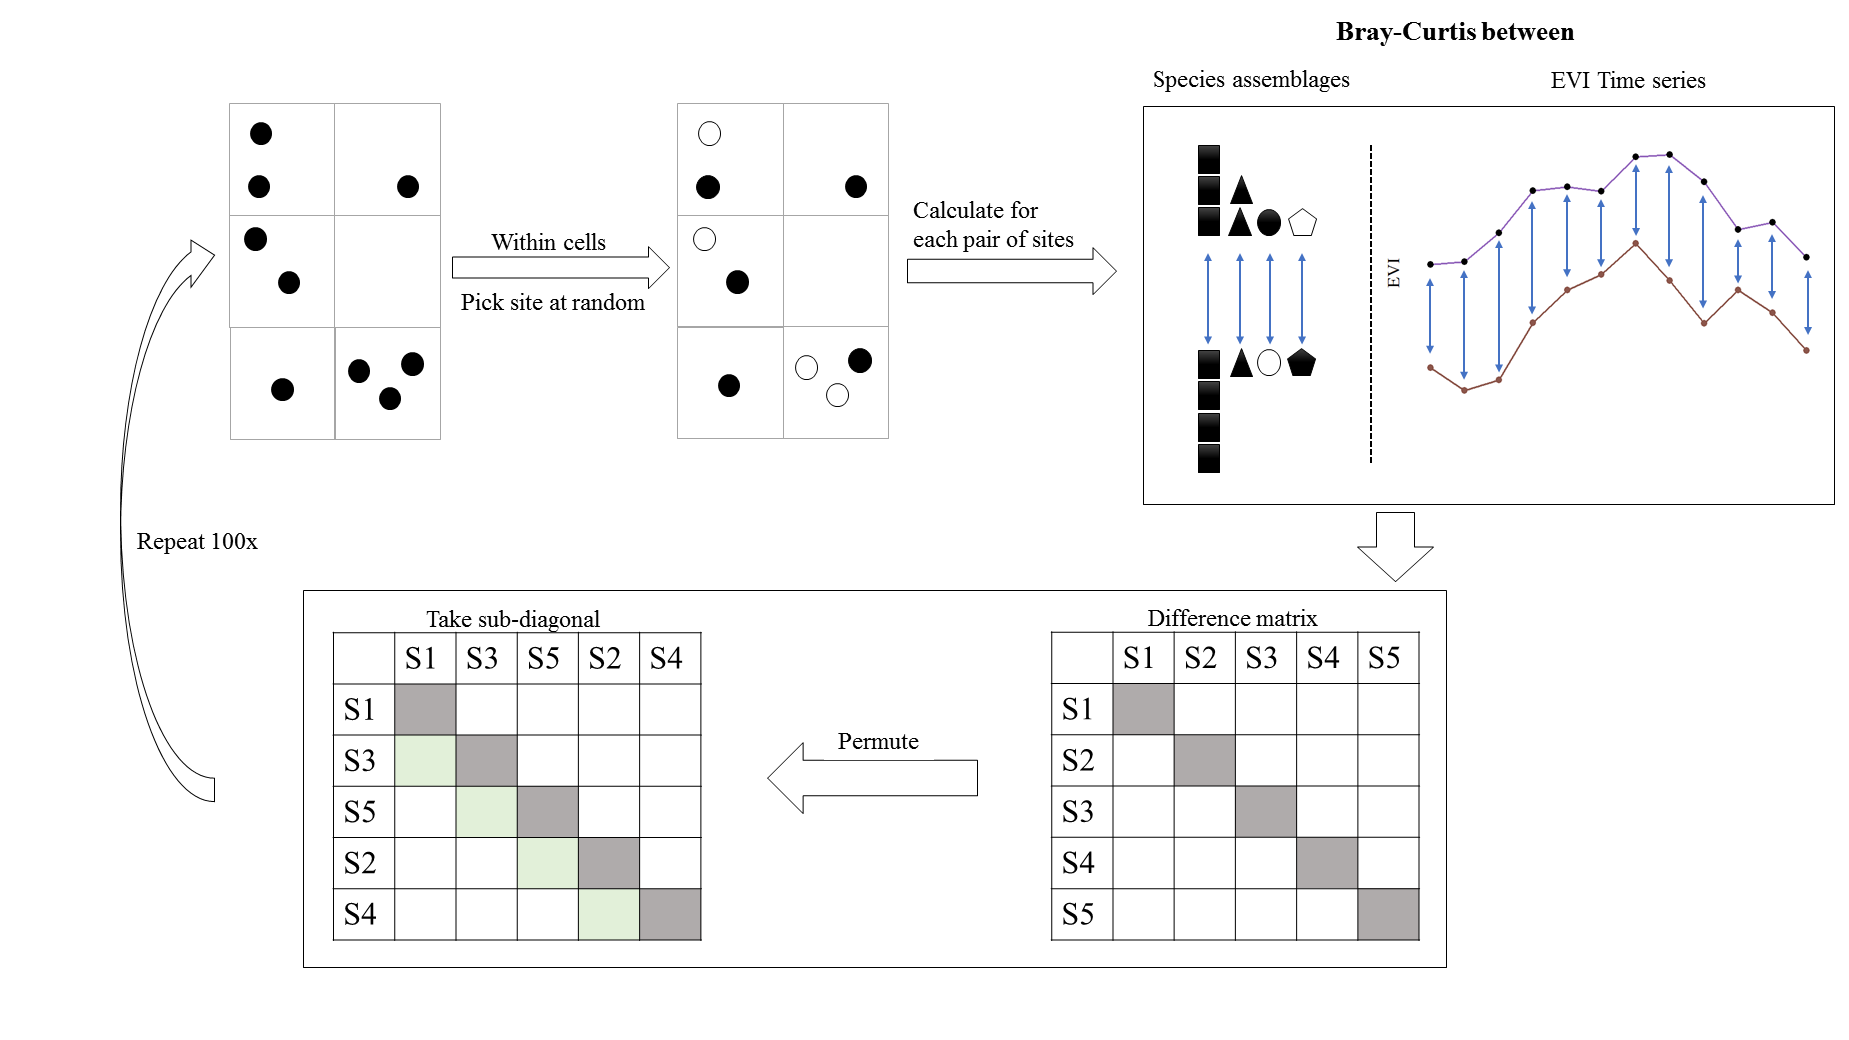
\includegraphics[width=1\textwidth]{chapter3/SI03}
\caption{ Correlations between attributes of abrupt land change. Showing shifts in magnitude, trend and time passed (see Methods). The lower facets show a point density plot, the upper facets the Pearson correlation coefficient between pairs of attributes and the diagonal a density plot.}
\label{SI03_03}
\end{figure}

%\endgroup
